\documentclass[11pt]{article}

% ----------------------------------------------------------------------------
% Parallelized Polynomial Root Finder -- explanatory write-up.
% Self-contained: all figures are TikZ (no external images). Compiles with
% pdflatex (run twice for cross-references) or on Overleaf.
% ----------------------------------------------------------------------------
\usepackage[margin=1in]{geometry}
\usepackage{amsmath,amssymb,amsthm}
\usepackage{tikz}
\usetikzlibrary{arrows.meta,calc,decorations.markings,positioning}
\usepackage{booktabs}
\usepackage{xcolor}
\usepackage{listings}
\usepackage{caption}
\usepackage[colorlinks=true,linkcolor=blue,urlcolor=blue,citecolor=blue]{hyperref}

\definecolor{live}{RGB}{174,214,241}
\definecolor{dead}{RGB}{245,245,245}
\definecolor{edgeH}{RGB}{192,57,43}
\definecolor{edgeV}{RGB}{31,97,141}
\definecolor{codebg}{RGB}{246,248,250}

\lstset{basicstyle=\ttfamily\small,backgroundcolor=\color{codebg},
        frame=single,rulecolor=\color{gray!40},breaklines=true,
        columns=fullflexible,xleftmargin=1em}

\newtheorem{theorem}{Theorem}
\newcommand{\C}{\mathbb{C}}
\newcommand{\Z}{\mathbb{Z}}
\DeclareMathOperator{\wind}{wind}

\title{\textbf{A Parallelized Polynomial Root Finder}\\[2pt]
       \large Subdivision and the Argument Principle on the GPU}
\author{Mohammed Ahmed}
\date{July 2026}

\begin{document}
\maketitle

\begin{abstract}
We describe a complex-analytic method for finding \emph{all} roots of a
polynomial by recursively subdividing a bounding square and counting the roots
in each sub-region with the \emph{argument principle} (winding numbers), then
polishing each isolated root with a multiplicity-aware Newton step. The method
is deliberately structured as a breadth-first work-list so that it maps directly
onto a GPU: each level of the search becomes one kernel launch over a grid of
independent cells. We present a CPU reference implementation and three GPU
variants that compute the same winding counts with progressively more
parallelism---a \emph{naive} per-cell scheme, a \emph{gather} scheme that shares
work between neighbouring cells via edge tables, and a \emph{scatter} scheme
that fuses the sharing using atomic accumulation. We benchmark all four against
NumPy's companion-matrix eigensolver and a multiprecision reference
(\texttt{mpmath}), and discuss the limitations---phantom roots, tightly
clustered and high-multiplicity roots, and catastrophic cancellation---that the
approach shares with, or improves upon relative to, industrial solvers.
\end{abstract}

% ============================================================================
\section{Introduction and Motivation}
% ============================================================================
Finding the roots of a polynomial
\[
  P(z) = c_n z^n + c_{n-1} z^{n-1} + \cdots + c_1 z + c_0, \qquad c_i \in \C,
\]
is one of the oldest and most ubiquitous problems in computation. Roots of
polynomials appear as the eigenvalues of matrices, the poles and zeros of
transfer functions in control theory and signal processing, the intersection
points of a ray with an implicit surface in computer graphics, and the
solutions of the kinematic equations in robotics. In many of these settings one
must solve not one but \emph{millions} of small polynomials---one per pixel, per
sample, or per configuration---which is precisely the regime where a graphics
processing unit (GPU), with its thousands of parallel threads, can dominate a
CPU.

The most widely used method today reformulates the problem as an eigenvalue
computation: the roots of $P$ are the eigenvalues of its \emph{companion matrix},
which one finds with a backward-stable QR iteration (this is what
\texttt{numpy.roots} and MATLAB's \texttt{roots} do). That approach is fast and
robust for a single polynomial of moderate degree, but it is inherently
sequential and computes \emph{all} $n$ roots whether or not they are wanted.

This report takes a different route, chosen because it \emph{parallelizes
naturally}. We enclose all roots in a square, subdivide it, and use a contour
integral---the argument principle---to count how many roots lie in each piece.
Because the count in each sub-square depends on nothing but that square's own
boundary, every sub-square can be processed by an independent thread. We develop
the idea on the CPU as a correctness oracle and then port it to the GPU in three
increasingly parallel forms.

We emphasize the scope of this work: the implementation here solves a
\emph{single} polynomial at a time. Batching many polynomials into one launch---
the setting sketched above, where the GPU most decisively beats the CPU---is a
natural extension that we identify as future work rather than a result we report
(Section~\ref{sec:limitations}).

% ============================================================================
\section{Background}
% ============================================================================
This section collects the classical results the method rests on. A reader
comfortable with complex analysis may skip to Section~\ref{sec:method}.

\subsection{The Fundamental Theorem of Algebra}
Every polynomial of degree $n \ge 1$ with complex coefficients has exactly $n$
roots in $\C$, counted with multiplicity
(\href{https://en.wikipedia.org/wiki/Fundamental_theorem_of_algebra}{FTA}). This
guarantees that our search is looking for a finite, known number of targets: the
counts we compute in each region must sum to $n$.

\subsection{Analytic Functions and Contours}
A polynomial is \emph{entire}: it is complex-differentiable everywhere and has no
poles. A \emph{contour} is a closed, oriented curve in $\C$; we always use the
boundary of an axis-aligned square, traversed counter-clockwise (CCW).

\subsection{The Argument Principle}
\label{sec:argprinciple}
The engine of the whole method is \emph{Cauchy's argument principle}
(\href{https://en.wikipedia.org/wiki/Argument_principle}{link}). For a function
$P$ analytic inside and on a contour $\Gamma$, with no zeros \emph{on} $\Gamma$,
\begin{equation}
  \frac{1}{2\pi i}\oint_{\Gamma} \frac{P'(z)}{P(z)}\,dz
  \;=\; N,
  \label{eq:argprinciple}
\end{equation}
where $N$ is the number of zeros of $P$ enclosed by $\Gamma$, counted with
multiplicity. Writing $P(z) = |P(z)|\,e^{i\arg P(z)}$, the integrand is
$\tfrac{d}{dz}\log P = \tfrac{d}{dz}\big(\log|P| + i\arg P\big)$, and the real
part integrates to zero around a closed loop. What survives is the change in the
\emph{argument}:
\begin{equation}
  N \;=\; \frac{1}{2\pi}\,\big[\text{total change in } \arg P(z)
          \text{ as } z \text{ traverses } \Gamma \text{ once CCW}\big]
      \;=\; \frac{1}{2\pi}\,\Delta_\Gamma \arg P.
  \label{eq:winding}
\end{equation}
In words: as $z$ walks once around the boundary, the image $P(z)$ winds around
the origin exactly $N$ times---the \emph{winding number} of $P\circ\Gamma$.
Figure~\ref{fig:argprinciple} illustrates this.

\begin{figure}[h]
\centering
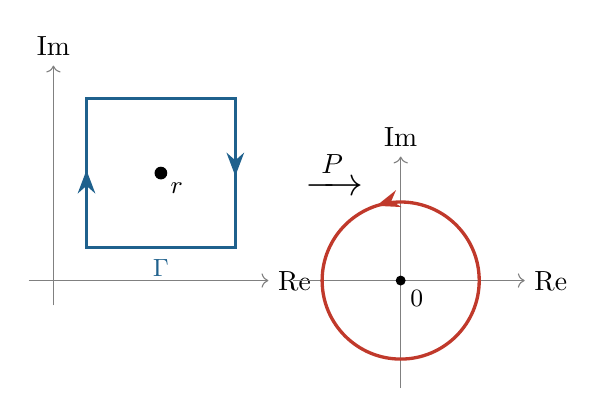
\begin{tikzpicture}[scale=1.05]
  % z-plane
  \begin{scope}
    \draw[->,gray] (-0.3,0)--(2.6,0) node[right,black]{$\mathrm{Re}$};
    \draw[->,gray] (0,-0.3)--(0,2.6) node[above,black]{$\mathrm{Im}$};
    \draw[very thick,edgeV,
      decoration={markings, mark=at position 0.13 with {\arrow{Stealth}},
                            mark=at position 0.63 with {\arrow{Stealth}}},
      postaction={decorate}]
      (0.4,0.4) rectangle (2.2,2.2);
    \filldraw[black] (1.3,1.3) circle (2pt) node[below right]{\small $r$};
    \node[edgeV] at (1.3,0.15) {\small $\Gamma$};
  \end{scope}
  % arrow
  \node at (3.4,1.3) {\Large $\xrightarrow{\;P\;}$};
  % w-plane
  \begin{scope}[xshift=4.2cm]
    \draw[->,gray] (-1.3,0)--(1.5,0) node[right,black]{$\mathrm{Re}$};
    \draw[->,gray] (0,-1.3)--(0,1.5) node[above,black]{$\mathrm{Im}$};
    \draw[very thick,edgeH,
      decoration={markings, mark=at position 0.30 with {\arrow{Stealth}}},
      postaction={decorate}]
      (0,0) circle (0.95);
    \filldraw[black] (0,0) circle (1.5pt) node[below right]{\small $0$};
  \end{scope}
\end{tikzpicture}
\caption{The argument principle. \emph{Left:} the $z$-plane contour $\Gamma$
enclosing a root $r$. \emph{Right:} its image $w=P(z)$, which winds around the
origin once for each enclosed root. Here $N=1$.}
\label{fig:argprinciple}
\end{figure}

\paragraph{Discrete winding.} We cannot integrate \eqref{eq:winding} exactly, so
we sample $S$ points $z_0,\dots,z_{S-1}$ around the boundary and accumulate the
change in argument between consecutive samples:
\begin{equation}
  \Delta_\Gamma \arg P \;\approx\; \sum_{k=0}^{S-1}
     \operatorname{unwrap}\!\big(\arg P(z_{k+1}) - \arg P(z_k)\big),
  \label{eq:discrete}
\end{equation}
where $\operatorname{unwrap}$ folds each increment into $(-\pi,\pi]$. Because
$\arg$ returns a principal value in an interval of width $2\pi$, consecutive raw
differences lie in $[-2\pi,2\pi]$, so a single $\pm 2\pi$ correction always
recovers the true (small) increment---\emph{provided the samples are dense
enough that the argument never truly changes by more than $\pi$ in one step}.
Dividing the total by $2\pi$ and rounding gives the integer count $N$.

\subsection{Root-Enclosing Bounds}
Before we can subdivide, we need an initial region guaranteed to contain every
root. Two classical bounds serve
(\href{https://en.wikipedia.org/wiki/Properties_of_polynomial_roots}{link}):
\begin{align}
  \text{Cauchy:} &\quad |z| \le 1 + \max_{0 \le k < n} \left|\frac{c_k}{c_n}\right|,\\
  \text{Fujiwara:} &\quad |z| \le 2\,\max_{1 \le k \le n}
     \left|\frac{c_{n-k}}{c_n}\right|^{1/k}, \text{ with the $k=n$ term halved.}
\end{align}
Both are valid upper bounds, so their minimum $R = \min(\text{Cauchy},
\text{Fujiwara})$ is too. Every root satisfies $|z| \le R$, so the square
$[-R,R]\times[-R,R]$ encloses all of them. (These bounds are themselves
Rouch\'e-type arguments: on a large enough circle the leading term $c_n z^n$
dominates the rest.)

\subsection{Newton's Method and Basins of Attraction}
Once a region has been narrowed to a single root, we refine it with
\emph{Newton's method}
(\href{https://en.wikipedia.org/wiki/Newton\%27s_method}{link}):
\begin{equation}
  z_{k+1} = z_k - \frac{P(z_k)}{P'(z_k)}.
\end{equation}
Newton converges quadratically near a simple root. However, its
\emph{basins of attraction}---the sets of starting points converging to each
root---are \emph{fractal}
(\href{https://en.wikipedia.org/wiki/Newton_fractal}{Newton fractal}): a seed
geometrically close to one root can converge to a distant one. This subtlety
turns out to matter (Section~\ref{sec:limitations}). For a root of multiplicity
$m$, the modified iteration $z_{k+1} = z_k - m\,P/P'$ restores quadratic
convergence.

% ============================================================================
\section{Method}
\label{sec:method}
% ============================================================================
The overall algorithm is a subdivision search:

\begin{enumerate}
  \item Compute the bound $R$ and start with the square $\Gamma_0 =
        [-R,R]\times[-R,R]$ (nudged by a tiny offset so no root lands exactly on
        a subdivision line, where the winding integral is undefined).
  \item Maintain a work-list of squares. For each square, compute its winding
        count $N$ via \eqref{eq:discrete}.
  \item \textbf{Triage} each square by its count:
    \begin{itemize}
      \item $N = 0$: no roots---\emph{discard} the square (a ``dead'' square).
      \item $N = 1$ and the square is small enough: the root is
        \emph{isolated}---send it to Newton polishing.
      \item $N \ge 2$ (or $N=1$ but still large): \emph{subdivide} the square
        into four and re-count each child.
    \end{itemize}
  \item Repeat until every surviving square is isolated, then polish.
\end{enumerate}

The invariant that makes the search sound is \emph{conservation}: by the
argument principle the counts of a square's four children must sum to the
parent's count, so no root is created or destroyed as we descend. Crucially, the
work at one level is a set of \emph{independent} winding computations---which is
exactly what a GPU wants.

\subsection{CPU Method}
The CPU reference uses \emph{binary} $2\times2$ subdivision driven by a
breadth-first work-list; each iteration of the outer \texttt{while} loop
processes one whole level. Two robustness features matter:
\begin{itemize}
  \item \textbf{Adaptive sampling.} The number of boundary samples starts at
    ${\sim}4n$ per side and \emph{doubles} whenever the computed winding is
    suspiciously far from an integer (a sign of undersampling near a grazing
    root).
  \item \textbf{Noise-floor trust.} When a square shrinks onto a multiple root,
    $|P|$ collapses toward the rounding-error floor $\varepsilon_{\text{mach}}
    \cdot (\text{largest Horner partial})$; there $\arg P$ is meaningless.
    Detecting this stops the search from ``burrowing into garbage.''
\end{itemize}
Figure~\ref{fig:subdiv} shows the subdivision as a quadtree over the complex
plane.

\begin{figure}[h]
\centering
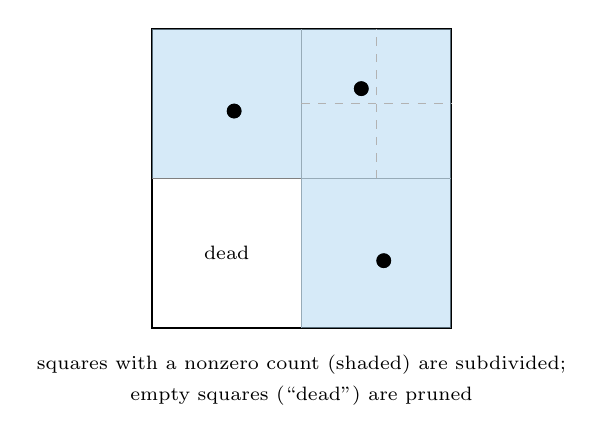
\begin{tikzpicture}[scale=1.9]
  % level-0 square
  \draw[thick] (0,0) rectangle (2,2);
  % level-1 split lines
  \draw[gray] (1,0)--(1,2); \draw[gray] (0,1)--(2,1);
  % roots
  \filldraw[black] (0.55,1.45) circle (1.3pt);
  \filldraw[black] (1.4,1.6) circle (1.3pt);
  \filldraw[black] (1.55,0.45) circle (1.3pt);
  % shade live quadrants (those containing roots) faintly
  \fill[live,opacity=0.5] (0,1) rectangle (1,2);   % NW: 1 root
  \fill[live,opacity=0.5] (1,1) rectangle (2,2);   % NE: 1 root
  \fill[live,opacity=0.5] (1,0) rectangle (2,1);   % SE: 1 root
  \node at (0.5,0.5) {\scriptsize dead};           % SW: 0 roots
  % re-draw roots on top
  \filldraw[black] (0.55,1.45) circle (1.3pt);
  \filldraw[black] (1.4,1.6) circle (1.3pt);
  \filldraw[black] (1.55,0.45) circle (1.3pt);
  % second-level split of NE (which we imagine has been chosen)
  \draw[gray!60,dashed] (1.5,1)--(1.5,2); \draw[gray!60,dashed] (1,1.5)--(2,1.5);
  \node[align=center] at (1,-0.35)
     {\scriptsize squares with a nonzero count (shaded) are subdivided;\\[-1pt]
      \scriptsize empty squares (``dead'') are pruned};
\end{tikzpicture}
\caption{Subdivision as a quadtree. Each square's winding count decides whether
it is pruned, subdivided, or handed to Newton.}
\label{fig:subdiv}
\end{figure}

\subsection{GPU Methods}
On the GPU, one level of the search is a grid of independent winding
computations. The three variants below all produce the \emph{same} per-cell
counts; they differ only in how they distribute the arithmetic. The dominant
cost in every case is evaluating $P$ (by Horner's method, $O(n)$ work) at each
of the ${\sim}S$ boundary samples of each cell.

\subsubsection{Naive Method}
The simplest scheme lays an $m\times m$ grid over the region and assigns
\textbf{one thread to one cell}. Each thread walks all four sides of its cell,
accumulates the argument change \eqref{eq:discrete}, and writes the integer
count. Cells with count $0$ are ``dead'' and dropped; cells with count $>0$ are
``live'' and passed to the next level. Figure~\ref{fig:naive} shows a grid with
its live and dead cells.

\begin{figure}[h]
\centering
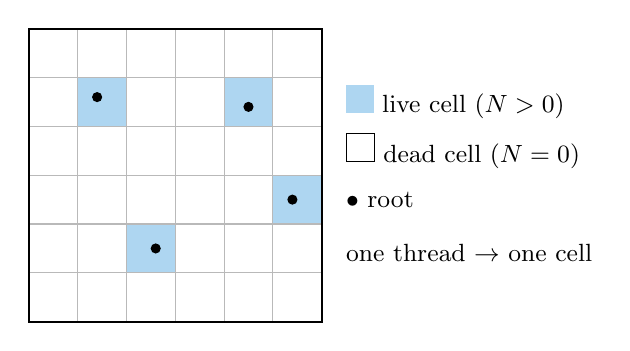
\begin{tikzpicture}[scale=0.62]
  \def\N{6}
  % roots (in grid coordinates 0..N)
  \coordinate (r1) at (1.4,4.6);
  \coordinate (r2) at (4.5,4.4);
  \coordinate (r3) at (2.6,1.5);
  \coordinate (r4) at (5.4,2.5);
  % shade the cells containing roots as "live"
  \foreach \p in {(1,4),(4,4),(2,1),(5,2)} { \fill[live] \p rectangle ++(1,1); }
  % grid
  \draw[step=1,gray!55] (0,0) grid (\N,\N);
  \draw[thick] (0,0) rectangle (\N,\N);
  % roots
  \foreach \r in {r1,r2,r3,r4} { \filldraw[black] (\r) circle (2.6pt); }
  % labels
  \node[anchor=west] at (\N+0.3,4.5) {\small \tikz\fill[live](0,0)rectangle(0.35,0.35); live cell ($N>0$)};
  \node[anchor=west] at (\N+0.3,3.5) {\small \tikz\draw(0,0)rectangle(0.35,0.35); dead cell ($N=0$)};
  \node[anchor=west] at (\N+0.3,2.5) {\small $\bullet$\ root};
  \node[anchor=west] at (\N+0.3,1.4) {\small one thread $\to$ one cell};
\end{tikzpicture}
\caption{Naive GPU winding. Each thread computes the winding count of one grid
cell independently. Shaded cells are ``live'' (contain roots) and survive to the
next level; the rest are pruned.}
\label{fig:naive}
\end{figure}

The naive scheme is simple but wasteful: every \emph{interior} edge of the grid
is shared by two adjacent cells, and each cell recomputes its own four edges. So
each interior edge---and the $O(n)$ Horner evaluations along it---is computed
\emph{twice}.

\subsubsection{Gather (H/V) Method}
The gather method removes that redundancy. Observe that an $m\times m$ grid has
about $4m^2$ cell-sides but only about $2m^2$ \emph{unique} edges (each interior
edge is shared). So we compute each unique edge \emph{once} and reuse it:

\begin{enumerate}
  \item \textbf{Edge pass.} One thread per unique edge. Each thread integrates
    the argument change along its edge (in a fixed canonical direction:
    horizontal edges left-to-right, vertical edges bottom-to-top) and stores the
    result---a real number, the edge's \emph{phase change}---in a table:
    $H[r][c]$ for horizontal edges, $V[r][c]$ for vertical edges.
  \item \textbf{Assembly pass.} One thread per cell. Each cell gathers its four
    edges from the tables and combines them with signs dictated by a CCW
    traversal:
    \begin{equation}
      N(r,c) = \operatorname{round}\!\left(
        \frac{H[r][c] + V[r][c{+}1] - H[r{+}1][c] - V[r][c]}{2\pi}\right).
      \label{eq:assemble}
    \end{equation}
\end{enumerate}
Because each edge is now evaluated once instead of twice, the gather method does
about \textbf{half} the Horner work of the naive method---the $2m^2$ vs.\ $4m^2$
ratio. It uses no atomics and is fully deterministic.
Figure~\ref{fig:gather} shows the shared edges and the four edges of one cell.

\begin{figure}[h]
\centering
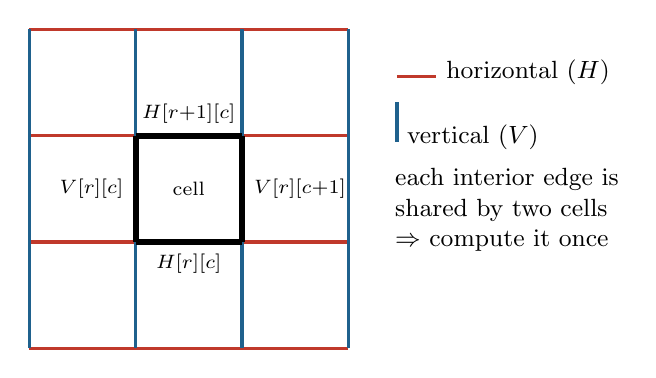
\begin{tikzpicture}[scale=1.35]
  \def\N{3}
  % grid cells
  \draw[step=1,gray!35] (0,0) grid (\N,\N);
  % highlight all horizontal edges and vertical edges by colour
  \foreach \y in {0,1,2,3} \foreach \x in {0,1,2}
     \draw[edgeH,line width=1.2pt] (\x,\y)--(\x+1,\y);
  \foreach \x in {0,1,2,3} \foreach \y in {0,1,2}
     \draw[edgeV,line width=1.2pt] (\x,\y)--(\x,\y+1);
  % the target cell (r=1,c=1) -> [1,2]x[1,2]; emphasize its 4 edges
  \draw[black,line width=2.2pt] (1,1)--(2,1) node[midway,below]{\scriptsize $H[r][c]$};
  \draw[black,line width=2.2pt] (2,1)--(2,2) node[midway,right]{\scriptsize $V[r][c{+}1]$};
  \draw[black,line width=2.2pt] (1,2)--(2,2) node[midway,above]{\scriptsize $H[r{+}1][c]$};
  \draw[black,line width=2.2pt] (1,1)--(1,2) node[midway,left]{\scriptsize $V[r][c]$};
  \node at (1.5,1.5) {\scriptsize cell};
  % legend
  \node[anchor=west] at (\N+0.35,2.6) {\small \tikz\draw[edgeH,line width=1.2pt](0,0)--(0.5,0); horizontal ($H$)};
  \node[anchor=west] at (\N+0.35,2.1) {\small \tikz\draw[edgeV,line width=1.2pt](0,0)--(0,0.5); vertical ($V$)};
  \node[anchor=west,align=left] at (\N+0.35,1.3)
    {\small each interior edge is\\[-1pt]\small shared by two cells\\[-1pt]
     \small $\Rightarrow$ compute it once};
\end{tikzpicture}
\caption{Gather method. Every unique edge (red $H$, blue $V$) is integrated once;
a cell's count is assembled from its four cached edges via \eqref{eq:assemble}.}
\label{fig:gather}
\end{figure}

\subsubsection{Scatter (Atomic) Method}
The scatter method achieves the same reuse but \emph{fuses} the two passes.
Instead of each cell \emph{gathering} its edges, each \textbf{edge thread}
computes its phase once and \emph{scatters} it into the two cells that share it,
via an atomic add. Using the CCW sign convention, a vertical edge adds $+$ to
the cell on its left and $-$ to the cell on its right; a horizontal edge adds $+$
to the cell above it and $-$ to the cell below (Figure~\ref{fig:scatter}). A
per-cell accumulator $M$ receives these contributions; a final pass divides by
$2\pi$ and rounds.

\begin{figure}[h]
\centering
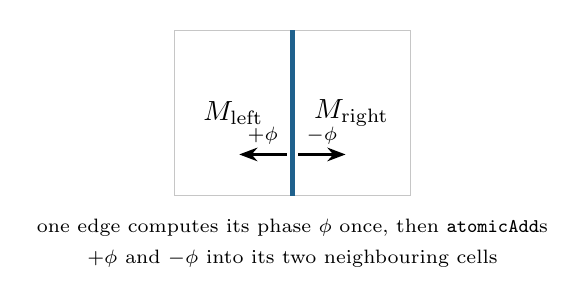
\begin{tikzpicture}[scale=1.5]
  % two cells sharing a vertical edge
  \draw[gray!45] (0,0) rectangle (1,1.4);
  \draw[gray!45] (1,0) rectangle (2,1.4);
  \draw[edgeV,line width=2pt] (1,0)--(1,1.4);
  \node at (0.5,0.7) {$M_{\text{left}}$};
  \node at (1.5,0.7) {$M_{\text{right}}$};
  \draw[-{Stealth},thick] (0.95,0.35) -- (0.55,0.35) node[midway,above]{\scriptsize $+\phi$};
  \draw[-{Stealth},thick] (1.05,0.35) -- (1.45,0.35) node[midway,above]{\scriptsize $-\phi$};
  \node[align=center] at (1,-0.4)
    {\scriptsize one edge computes its phase $\phi$ once, then \texttt{atomicAdd}s\\[-1pt]
     \scriptsize $+\phi$ and $-\phi$ into its two neighbouring cells};
\end{tikzpicture}
\caption{Scatter method. Each edge scatters its phase into the two cells it
borders with opposite signs; the assembly is fused into the scatter.}
\label{fig:scatter}
\end{figure}

\paragraph{Scatter vs.\ gather trade-off.} Scatter needs \emph{less memory}: it
keeps only the per-cell accumulator $M$ ($m^2$ numbers) rather than the two edge
tables $H$ and $V$ ($\approx 2m^2$ numbers), and it avoids a separate assembly
kernel. The cost is \emph{determinism}: atomic additions arrive in a
nondeterministic order, and floating-point addition is \emph{not associative}
(the rounding of $a+b+c$ depends on the order), so the accumulated $M$---and, at
a rounding boundary, the final count---can wobble in the last bits from run to
run. For well-conditioned inputs this is invisible; near a multiple root, where
the counts are already unreliable, the two schemes can even disagree.

% ============================================================================
\section{Results}
% ============================================================================
We benchmarked the CPU solver and the three GPU variants against
\texttt{numpy.roots} (a LAPACK companion-matrix eigensolver---the practical
baseline) and \texttt{mpmath.polyroots} (arbitrary precision---an accuracy
oracle). All methods share one input/output contract and run in the same
environment. Table~\ref{tab:results} shows representative cases; ``LOST'' means
a true root was dropped, and errors are the worst distance to a true root.

\begin{table}[h]
\centering
\small
\begin{tabular}{llrrr}
\toprule
Polynomial & Method & Roots found & Max error & Time (ms) \\
\midrule
Roots of unity, $z^{50}-1$ & CPU        & 50 / 50 & $9\!\times\!10^{-16}$ & $3260$ \\
                           & GPU (gather)& 50 / 50 & $9\!\times\!10^{-16}$ & $43$   \\
                           & NumPy      & 50 / 50 & $2\!\times\!10^{-15}$ & $2.0$  \\
                           & mpmath     & 50 / 50 & $9\!\times\!10^{-16}$ & $1650$ \\
\midrule
Wilkinson, $\prod_{k=1}^{20}(z-k)$ & CPU   & \textbf{LOST} (3) & --- & $146$ \\
                           & GPU (gather)& 20 / 20 & $9\!\times\!10^{-3}$ & $12$   \\
                           & NumPy      & 20 / 20 & $2\!\times\!10^{-2}$ & $0.6$  \\
                           & mpmath     & 20 / 20 & $6\!\times\!10^{-4}$ & $435$  \\
\midrule
Tight cluster (gap $10^{-6}$) & CPU     & 4 / 4 & $4\!\times\!10^{-8}$ & $3$ \\
                           & GPU (gather)& 4 / 4 & $9\!\times\!10^{-12}$ & $6$   \\
                           & NumPy      & 4 / 4 & $1\!\times\!10^{-10}$ & $0.3$  \\
\bottomrule
\end{tabular}
\caption{Representative benchmark results. The three GPU variants return
identical roots and differ only in speed (gather shown).}
\label{tab:results}
\end{table}

Three findings stand out.
\begin{itemize}
  \item \textbf{The GPU is far faster than the CPU} on well-conditioned
    problems---roughly $10$--$75\times$ at these degrees (e.g.\ $43$\,ms vs.\
    $3260$\,ms at degree $50$)---validating the port against its own baseline.
  \item \textbf{NumPy remains the overall winner} at these degrees: it is the
    fastest \emph{and} robust. The GPU's fixed launch and data-transfer overhead
    means it can only overtake NumPy at much higher degree, or---its natural
    regime---when solving many polynomials in a single \emph{batch}.
  \item \textbf{The subdivision method is often \emph{more robust} than the CPU's
    own weaknesses would suggest}, and on several hard cases (Wilkinson, tight
    clusters, wide dynamic range) the finer GPU grid recovers roots the CPU
    drops.
\end{itemize}
Among the three GPU variants the counts are identical, so accuracy is the same;
the differences are purely in speed, where the gather scheme's elimination of
redundant edge work makes it the fastest of the three at scale.

% ============================================================================
\section{Limitations}
\label{sec:limitations}
% ============================================================================
The method has real limitations, most of which trace back to the finite
precision of floating-point arithmetic.

\paragraph{Phantom roots.} Near a high-multiplicity root, $|P|\sim r^m$ collapses
toward the rounding-noise floor before the enclosing square becomes small. There
$\arg P$ is dominated by round-off, so the discrete winding integral
\eqref{eq:discrete} returns a \emph{wrong} integer. In the worst case the search
subdivides noise into spurious ``phantom'' boxes---for example $(z-1)^{24}$ can
report a total multiplicity of $42$ instead of $24$---or loops until a work-list
cap halts it. A cap guarantees termination, but a genuinely robust fix requires
raising the noise floor (compensated Horner) or replacing the integer winding
with a \emph{certified} count via Rouch\'e/Pellet tests, which fail \emph{safe}
(inconclusive $\to$ subdivide) rather than fail \emph{wrong}.

\paragraph{Clusters and high multiplicity.} A root of multiplicity $m$ is
intrinsically ill-conditioned: perturbing the coefficients by $\varepsilon$ moves
the root by ${\sim}\varepsilon^{1/m}$. In double precision this caps the
achievable accuracy at ${\sim}\varepsilon_{\text{mach}}^{1/m}$---about
$10^{-8}$ for a double root, $10^{-5}$ for a triple. This limit is
\emph{universal}: NumPy hits the same ceiling. The difference is the failure
\emph{mode}---the companion-matrix method degrades gracefully (it always returns
$n$ points, just imprecise ones), whereas subdivision can \emph{miscount} at the
noise floor.

\paragraph{Catastrophic cancellation.} When the roots span a wide dynamic range
(say $10^{-3}$ to $10^{3}$), Horner evaluation near the small roots suffers
catastrophic cancellation: the partial sums are large while $|P|$ is tiny, so the
relative error explodes and $\arg P$ becomes unreliable. Empirically the method
tolerates only ${\sim}2$--$3$ orders of magnitude of spread. Wilkinson's
polynomial $\prod_{k=1}^{20}(z-k)$
(\href{https://en.wikipedia.org/wiki/Wilkinson\%27s_polynomial}{link}) is the
canonical example of this coefficient ill-conditioning, and it defeats every
double-precision method to some degree.

\paragraph{A Newton-basin pitfall.} Isolating a single-root cell does not
guarantee Newton converges to \emph{that} root: because Newton basins are
fractal (Section~2.5), a seed at the cell's centre can escape across a basin
boundary to a neighbouring root---catastrophically so for symmetric, densely
packed roots like roots of unity. The fix is to subdivide until the cell is small
enough (a threshold that must shrink like $1/n$ with the degree) that the centre
is safely inside the correct basin.

\paragraph{GPU utilization.} A single small polynomial simply does not contain
enough parallel work to fill a GPU: a degree-$50$ solve has only ${\sim}50$
active cells per level, far short of the tens of thousands of threads a GPU wants
resident. The method's true GPU regime is therefore \emph{batch throughput}
(many polynomials at once) and very high degree---not single-polynomial latency,
which is the GPU's least favourable framing. This work does \emph{not} yet
implement batching: every solve here processes one polynomial, and turning the
per-polynomial pipeline into a single batched launch is the most promising line
of future work.

% ============================================================================
\section{References}
% ============================================================================
\begin{itemize}
  \item Cauchy's argument principle ---
    \url{https://en.wikipedia.org/wiki/Argument_principle}
  \item Fundamental theorem of algebra ---
    \url{https://en.wikipedia.org/wiki/Fundamental_theorem_of_algebra}
  \item Bounds on polynomial roots (Cauchy, Fujiwara) ---
    \url{https://en.wikipedia.org/wiki/Geometrical_properties_of_polynomial_roots}
  \item Newton's method and Newton fractals ---
    \url{https://en.wikipedia.org/wiki/Newton_fractal}
  \item Wilkinson's polynomial (ill-conditioning) ---
    \url{https://en.wikipedia.org/wiki/Wilkinson\%27s_polynomial}
  \item Rouch\'e's and Pellet's theorems (certified root counting) ---
    \url{https://en.wikipedia.org/wiki/Rouch\%C3\%A9\%27s_theorem}
  \item D.~A.~Bini and G.~Fiorentino, \emph{Design, analysis, and implementation
    of a multiprecision polynomial rootfinder} (MPSolve), Numer.\ Algorithms,
    2000.
  \item Companion matrix / eigenvalue method (as used by
    \texttt{numpy.roots}) ---
    \url{https://en.wikipedia.org/wiki/Companion_matrix}
\end{itemize}

\end{document}
